%----------------------------------------------------------------------------------------
%	PACKAGES AND THEMES
%----------------------------------------------------------------------------------------
\documentclass[aspectratio=169,xcolor=dvipsnames, t]{beamer}
\usepackage{fontspec} % Allows using custom font. MUST be before loading the theme!
\usetheme{SimplePlusAIC}
\usepackage{hyperref}
\usepackage{graphicx} % Allows including images
\usepackage{booktabs} % Allows the use of \toprule, \midrule and  \bottomrule in tables
\usepackage{svg} %allows using svg figures
\usepackage{tikz}
\usepackage{makecell}
\usepackage{wrapfig}
\usepackage{algorithm}
\usepackage{algorithmic}
\usepackage[style=ieee]{biblatex}
\addbibresource{ref_enkf.bib}

% ADD YOUR PACKAGES BELOW

%----------------------------------------------------------------------------------------
%	TITLE PAGE CONFIGURATION
%----------------------------------------------------------------------------------------

\title[the Ensemble Kalman Filter (EnKF)]{the Ensemble Kalman Filter (EnKF)} 

\author[N. ZAOUACHE]{Narimane ZAOUACHE \\[5mm]{\small Supervisor: M. Christophe PRUD’HOMME}}

\institute[]{University of Strasbourg}

\date{\today} % Date, can be changed to a custom date
%----------------------------------------------------------------------------------------
%	PRESENTATION SLIDES
%----------------------------------------------------------------------------------------

\begin{document}

\maketitlepage

\begin{frame}[t]{Overview}
    \tableofcontents
\end{frame}

%------------------------------------------------
% Section divider frame
\makesection{Contexte and Objectives}

%------------------------------------------------
% Bullets
\begin{frame}{Context}
    Study of the application of the Ensemble Kalman Filter (EnKF) to nonlinear dynamic systems, specifically the Lorenz system.
\begin{block}{}
    The Ensemble Kalman Filter\cite{wikipediaEnKF} is a powerful tool for state estimation in nonlinear and high-dimensional systems, enhancing forecast accuracy by integrating observational data.

\end{block}


\end{frame}

%------------------------------------------------
% Lists
\begin{frame}{Objectives}
    \begin{enumerate}
        \item To determine how effective the Ensemble Kalman Filter (EnKF) is in tracking and predicting the behavior of the Lorenz system, which is intrinsically chaotic.
        \item To examine how different parameters, such as observation noise levels and ensemble size, influence the performance of the EnKF in forecasting the future states of the system.
    \end{enumerate}
\end{frame}

%------------------------------------------------
% Section divider frame
\makesection{Background}

%------------------------------------------------
\begin{frame}{Lorenz system and ODEs solvers}
    \begin{columns}
\begin{column}{0.5\textwidth}
  \begin{center}
\large
\[
\begin{cases}
    \displaystyle\frac{dx}{dt} = \sigma(y - x) \\
    \displaystyle\frac{dy}{dt} = x(\rho - z) - y \\
    \displaystyle\frac{dz}{dt} = xy - \beta z
\end{cases}
\]
  \end{center}
   
\end{column}
\begin{column}{0.5\textwidth}  %%<--- here
    where:\cite{lorenz}
\begin{itemize}
    \item $x$ is the rate of convective overturning,  \cite{lorenz}
    \item $y$ is the horizontal temperature variation,
    \item $z$ is the vertical temperature variation,
    \item $\sigma $ is the Prandtl number,
    \item $\rho $ is the Rayleigh number,
    \item $\beta $ is a geometrical factor.
\end{itemize}
\end{column}
\end{columns}
\end{frame}

\begin{frame}{Explicit Euler Method}
    \begin{columns}
        \begin{column}{0.5\textwidth}
            \textbf{Method Description:}
            \begin{itemize}
                \item Simple and effective for step-by-step approximation.
                \item Uses the derivative to estimate state changes.
            \end{itemize}
        \end{column}
        
        \begin{column}{0.5\textwidth}
            \begin{figure}
                \centering
                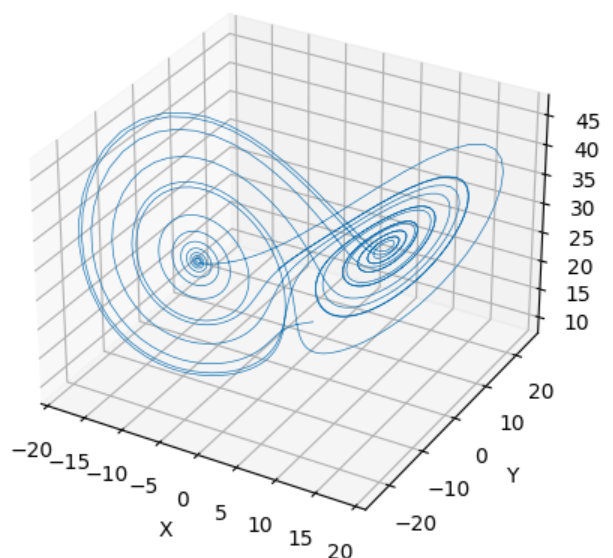
\includegraphics[width=.75\textwidth]{figures/lorenz_euler.png}
                \caption{Lorenz system solved with Explicit Euler}
                \label{fig:lorenz_euler}
            \end{figure}
        \end{column}
    \end{columns}
\end{frame}

\begin{frame}{Ensemble Kalman Filter (EnKF)}
The Ensemble Kalman Filter \cite{labbe2020} works by :

\begin{itemize}
    \item \textbf{Propagation through the Model}
we use our dynamic model to predict future states by running multiple state samples through it.
\\
    \item \textbf{Update with Observations}
we adjust these predictions based on actual observations to get a more accurate estimate of the system’s state.
\end{itemize}
\end{frame}

%------------------------------------------------
% Section divider frame
\makesection{Implementation and Results}

%------------------------------------------------

\begin{frame}{EnKF Algorithm Steps}

    \textbf{1. Initialization:} Generate initial state samples \(\{x_i^0\}_{i=1}^N\).

    \textbf{2. Prediction:} Forecast the next state for each ensemble member \cite{iglesias2013ensemble}:
    \[
    x_i^{\text{pred}} = f(x_i^{\text{upd}}) + w_i
    \]

    \textbf{3. Update:} Adjust predictions based on observations:
    \begin{itemize}
        \item Compute predicted observation:
        \[
        z_i^{\text{pred}} = h(x_i^{\text{pred}}) + v_i
        \]
        \item Calculate Kalman gain:
        \[
        K_k = P_k^{\text{pred}} H^T (H P_k^{\text{pred}} H^T + R)^{-1}
        \]
        \item Update state estimates:
        \[
        x_i^{\text{upd}} = x_i^{\text{pred}} + K_k (z_k - h(x_i^{\text{pred}}))
        \]
    \end{itemize}
\end{frame}


\begin{frame}{Results}
\textbf{EnKF Trajectories and Deviations}
    \begin{figure}[ht!]
        \centering
        \resizebox{0.45\textwidth}{!}{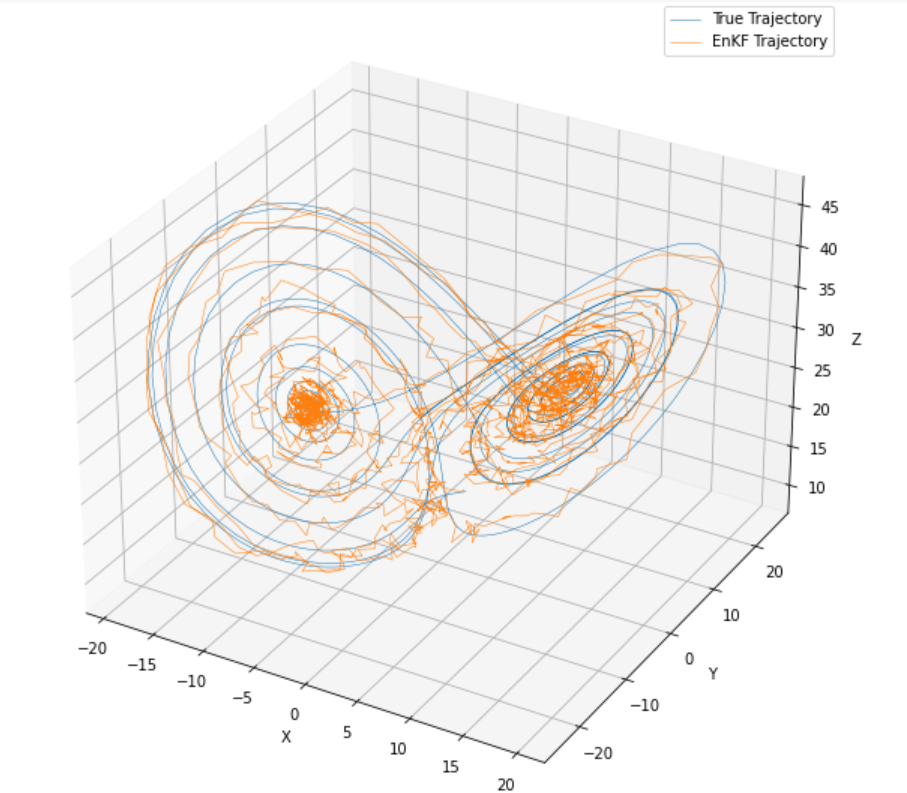
\includegraphics{figures/lorenz_enkf.png}}
        \caption{Lorenz system with EnKF}
        \label{fig:2}
     \end{figure}   
\end{frame}

\begin{frame}{Results}
\textbf{Uncertainty of Estimates and Absolute Errors}
    \begin{columns}
\begin{column}{0.5\textwidth}
   \begin{figure}[ht!]
    \centering
    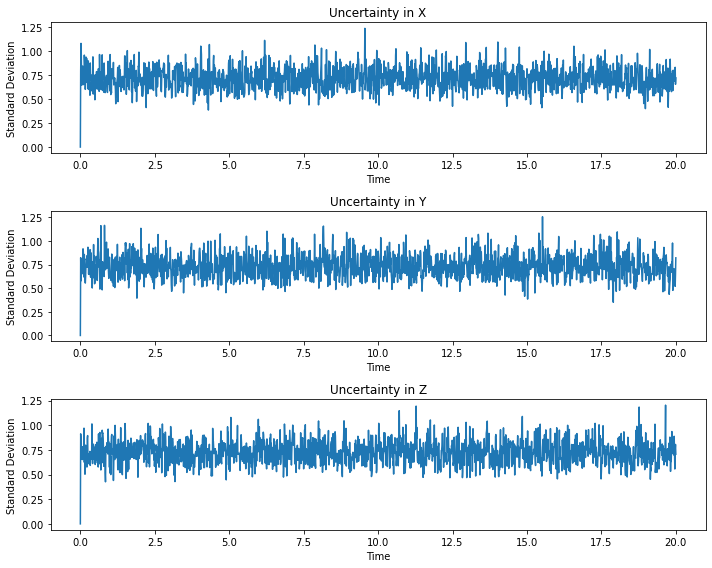
\includegraphics[width=0.8\textwidth]{figures/incertitude.png}
    \caption{Uncertainty}
    \label{fig:3}
\end{figure}
\end{column}
\begin{column}{0.5\textwidth}  %%<--- here
    \begin{center}
     \begin{figure}[ht!]
    \centering
    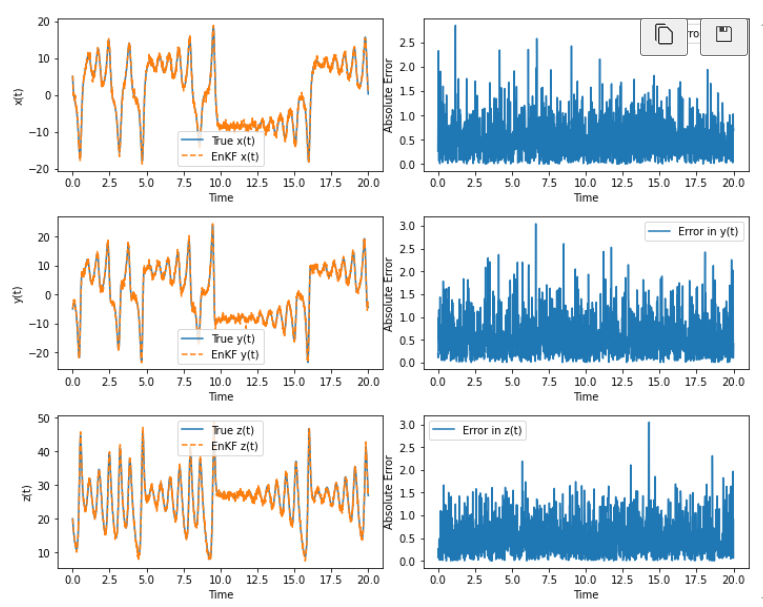
\includegraphics[width=0.7\textwidth]{figures/erreur_abs.png}
    \caption{Individual Trajectories and Absolute Errors}
    \label{fig:4}
\end{figure}
     \end{center}
\end{column}
\end{columns}
    
\end{frame}

\begin{frame}{Results}
\textbf{Impact of Observation Covariance Matrix ($R$)}
    \begin{figure}[ht!]
        \centering
        \resizebox{0.7\textwidth}{!}{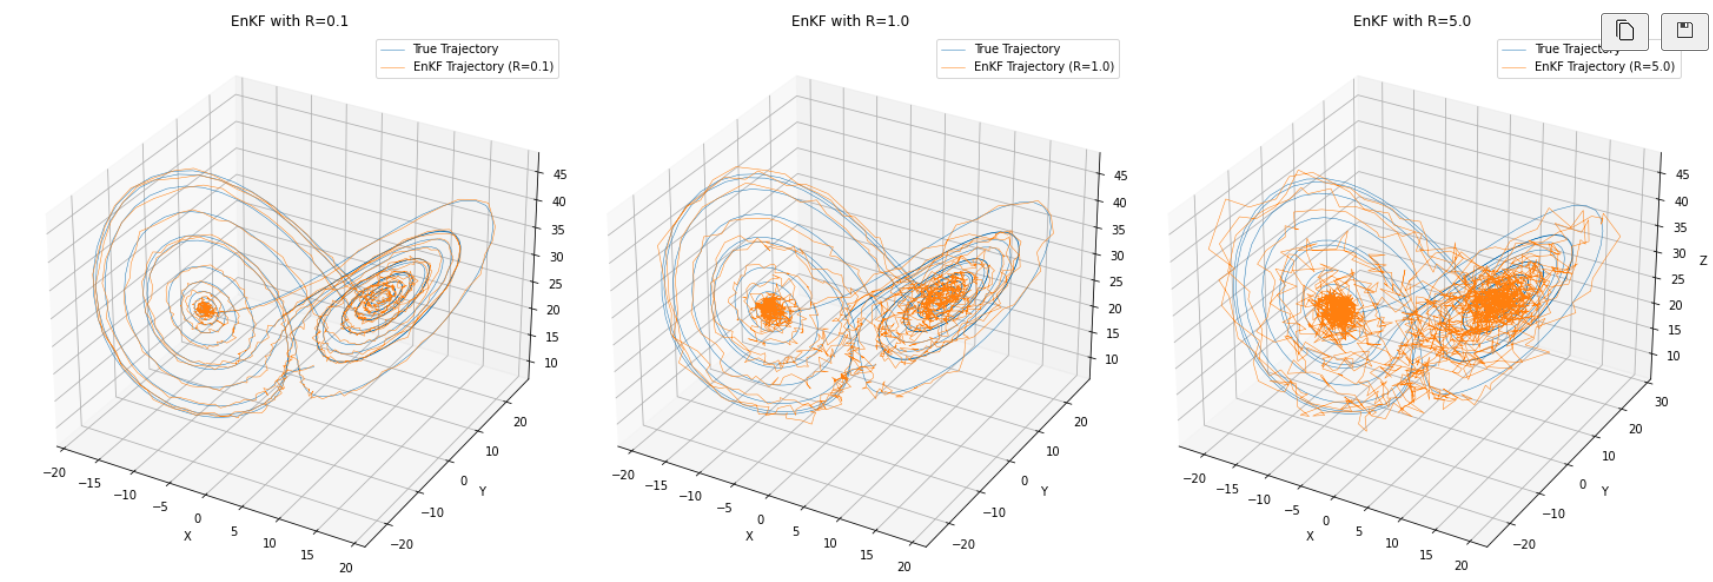
\includegraphics{figures/Matrice_d_observation.png}}
        \caption{Lorenz System Analysis Using Ensemble Kalman Filter for Different R Values}
        \label{fig:5}
     \end{figure}  
\end{frame}


 \begin{frame}{Results}
 \textbf{Impact of Ensemble Size ($N$)}
    \begin{figure}[ht!]
        \centering
        \resizebox{0.7\textwidth}{!}{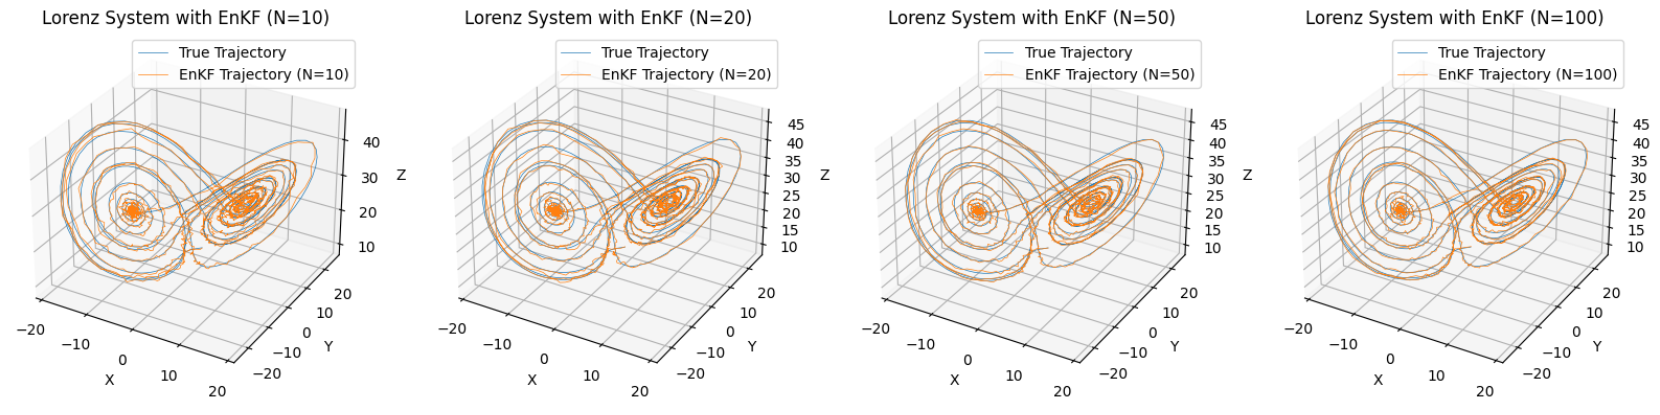
\includegraphics{figures/ensemble_N.png}}
        \caption{Influence of the Number of Ensembles N}
        \label{fig:6}
     \end{figure}  
\end{frame}   

% Section divider frame
\makesection{Conclusion}
\begin{frame}{Conclusion}
\textbf{Effectiveness of EnKF:}
\begin{itemize}
    \item The Ensemble Kalman Filter (EnKF) has proven effective in estimating the states of the Lorenz system, even in the presence of uncertainties and noise.
\end{itemize}
\textbf{Sensitivity to Parameters:}
\begin{itemize}
    \item The performance of the EnKF is influenced by observation noise levels and ensemble size.
\end{itemize}
\end{frame}

%------------------------------------------------
% Refenrenced
\begin{frame}[allowframebreaks]{References}
    %\nocite{*}
    \printbibliography
	
\end{frame}

%----------------------------------------------------------------------------------------
% Final PAGE
% Set the text that is showed on the final slide
\finalpagetext{Thank you for your attention}
%----------------------------------------------------------------------------------------
\makefinalpage
%----------------------------------------------------------------------------------------
\end{document}